\section{Implementasi}

Bagian ini akan menjelaskan tentang implementasi sistem \textit{remote deployment} secara terperinci. Seperti yang telah dijelaskan pada  \textbf{Bagian \ref{sec:rancangan-dashboard}} dan \textbf{\ref{sec:rancangan-service}} terdapat dua komponen utama yaitu \textit{dashboard} dan \textit{service}. Penjelasan bagian ini akan dimulai dari batasan implementasi, dilanjutkan dengan kakas yang digunakan dalam proses pembuatan sistem dan diakhiri dengan penjelasan mengenai implementasi dari \textit{dashboard} dan \textit{service}

\subsection{Batasan Implementasi}
Berikut adalah batasan yang ditetapkan dalam melakukan implementasi \textit{sistem remote deployment}.

\begin{enumerate}
  \item Semua batasan masalah dan konfigurasi yang telah dibahas pada bagian \ref{sec:batasan-masalah}.
  \item Kubernetes cluster berjalan di lokal dengan menggunakan kakas \textit{kind} dan hanya dibatasi menjadi 4 node dengan spesifikasi \textit{1 master} dan \textit{3 worker}
  \item \textit{Device} sudah terkoneksi sebelumnya sehingga tidak perlu register \textit{device} dan menghubungkannya ke dalam \textit{cluster}.
\end{enumerate}

\subsection{Kakas yang Digunakan}
Dalam melakukan implementasi ini diperlukan beberapa kakas, diantaranya adalah sebagai berikut.
\begin{enumerate}
  \item \textit{Docker}, \textit{Docker Desktop} dan \textit{Kind} untuk dipakai sebagai \textit{containerization} dan \textit{cluster} kubernetes lokal.
  \item Implementasi \textit{service} bahasa pemrograman golang dan menggunakan beberapa kakas berikut
        \begin{enumerate}
          \item \textit{Kubernetes Go Client} untuk mengontrol \textit{cluster} kubernetes melalui kode Golang.
          \item \textit{Echo} sebagai \textit{server framework}
          \item \textit{Logrus} sebagai logger dari setiap aksi pada sistem
          \item \textit{Cobra dan Viper} sebagai \textit{CLI command} pada golang untuk memudahkan pemilihan \textit{entrypoint} dan \textit{environment variables}
          \item \textit{PQ, Sqlx, Go-migrate} sebagai kakas yang menghubungkan sistem dengan database. Sqlx merupakan ekstensi dari library \textit{database/sql} milik golang. Go migrate digunakan untuk melakukan migrasi dari schema sql yang telah dibuat dan melakukan keep track dari versi schema yang sedang digunakan
          \item \textit{Validator} digunakan untuk memvalidasi \textit{request} yang masuk
        \end{enumerate}

  \item Implementasi \textit{dashboard} menggunakan \textit{vue} dan \textit{typescript} dan \textit{nuxt} sebagai framework.
        \begin{enumerate}
          \item \textit{NuxtUI} Sebagai kakas untuk memudahkan pembuatan \textit{UI}.
          \item \textit{Pinia} Sebagai kakas untuk manajemen data \textit{UI}.
          \item \textit{Zod} Sebagai object schema validator sebelum mengirimkan request.
        \end{enumerate}
\end{enumerate}

\subsection{Persiapan \textit{kubernetes cluster}}
\label{subsec:persiapan-kubernetes-cluster}

Tahapan ini merupakan tahapan persiaspan sebelum proses \textit{development}. Pada tahapan ini dibuat kubernetes \textit{cluster} pada komputer lokal dengan kakas \textit{kind}. \textit{Cluster} yang dibuat memiliki 4 nodes dengan spesifikasi 1 \textit{master node} dan 3 \textit{worker node}. Digunakan \textit{command} kind create cluster --config cluster.yaml dengan file konfigurasi yang dapat dilihat pada gambar \ref{fig:konfigurasi-pembuatan-cluster}. Setelah berhasil di \textit{apply}, muncul 4 buah kontainer yang dapat berfungsi sebagai \textit{kubernetes cluster} seperti pada gamabar \ref{fig:hasil-cluster-kind}

\begin{figure}[ht]
  \centering
  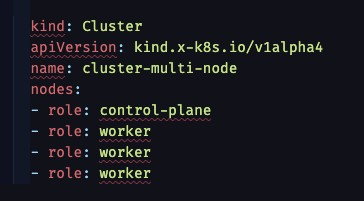
\includegraphics[width=1\textwidth]{resources/appendix/pembuatan-cluster.jpg}
  \caption{Konfigurasi Pembuatan \textit{Kubernetes Cluster} Dengan Kakas \textit{Kind}}
  \label{fig:konfigurasi-pembuatan-cluster}
\end{figure}

\begin{figure}[ht]
  \centering
  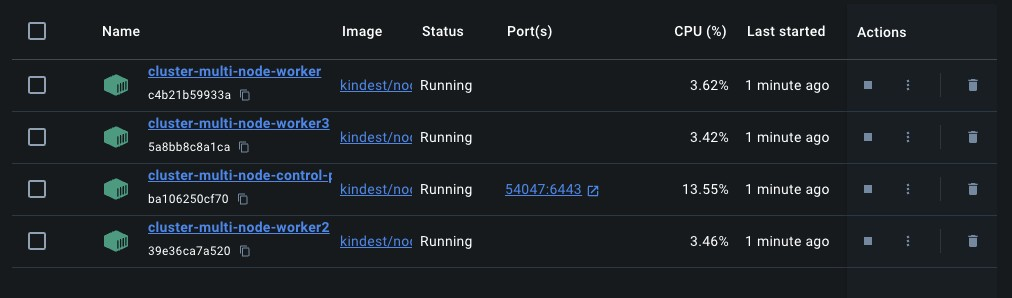
\includegraphics[width=1\textwidth]{resources/chapter-4/cluster-kind.jpg}
  \caption{Hasil \textit{Kubernetes Cluster} Dengan Kakas \textit{Kind}}
  \label{fig:hasil-cluster-kind}
\end{figure}

\pagebreak

\subsection{Implementasi \textit{Dashboard}}
komponen \textit{dashboard} dibuat dengan menggunakan bahasa pemrogramman \textit{typescript} dan \textit{vue}. Framework yang digunakan dalam membuat \textit{Dashboard} adalah \textit{Nuxt}. \textit{Nuxt} menjadi pilihan karena memiliki \textit{developer experience} yang bagus serta fitur yang cukup lengkap. \textit{Nuxt} juga memiliki \textit{UI library} yaitu \textit{NuxtUI} yang memudahkan pembuatan \textit{UI}. Pada komponen ini, terdapat 13 halaman yang dapat dikunjungi oleh \textit{user}. Detail dari penjelasan setiap halaman dapat ditemukan pada subbab dibawah ini.

\subsubsection{Halaman \textit{Login}}
Halaman ini berada pada \textit{route} \textbf{/login}. Halaman ini yang berfungsi sebagai \textit{entrypoint} dari komponen \textit{dashboard}. Pada halaman ini terdapat dua input yang di \textit{wrap} oleh sebuah \textit{form}. Input berupa \textit{email} dan \textit{password} \textit{user}. Setelah \textit{user} memasukan \textit{email} dan \textit{password} yang sesuai, maka akan dilakukan \textit{redirect} ke laman utama untuk menunjukan bahwa \textit{user} berhasil terautentikasi dan menggunakan fungsionalitas \textit{dashboard}. Tampilan halaman ini dapat dilihat pada gambar \ref{fig:halaman-login}

\subsubsection{Halaman utama}
Halaman ini merupakan halaman utama dari komponen \textit{dashboard}. Pada halaman ini \textit{user} dapat melihat status dari masing masing objek mulai dari \textit{deployment}, \textit{device}, \textit{group}, serta \textit{quick actions} untuk menuju halaman terkait.

\subsubsection{Halaman \textit{Account}}
Halaman ini berada pada \textit{route \textbf{/account}}. Halaman ini berfungsi untuk memberikan detail mengenai \textit{company} dari \textit{user}. Informasi \textit{company} ditampilkan pada sebuah \textit{card} yang berada pada tengah halaman. Pada halaman ini juga ditampilkan informasi mengenai daftar \textit{user} yang berada pada \textit{company} yang sama dan ditampilkan dengan sebuah tabel. Tampilan halaman ini dapat dilihat pada gambar \ref{fig:halaman-account}

\subsubsection{Halaman \textit{Device}}
Halaman ini berada pada \textit{route \textbf{/devices}}. Halaman ini berfungsi untuk melakukan manajemen \textit{device} pada satu perusahaan. Halaman ini menunjukan informasi seluruh \textit{device} yang terdaftar pada \textit{company}. Tampilan halaman ini dapat dilihat pada gambar \ref{fig:halaman-device}

Sama seperti halaman \textit{account}, terdapat tombol dengan icon elipsis pada bagian kanan untuk melakukan fungsi seperti melihat detail ataupun menghapus \textit{device} terkait. Apabila \textit{user} menekan tombol \textit{detail} maka user akan diarahkan ke halaman \textbf{/device/:id} sesuai dengan id \textit{device} yang dipilih. Tombol yang dimaksud dapat dilihat pada gambar \ref{fig:halaman-device-actions}

Pada halaman ini terdapat tombol yang dapat ditekan untuk menambahkan \textit{device}. Apabila ditekan akan muncul sebuah modal. Modal ini berisi input yang dapat \textit{user} isi untuk membuat sebuah \textit{device} baru pada sistem. Terdapat validasi pada setiap input, setelah semua validasi dilewati, tombol \textit{submit} akan mengirimkan \textit{request} ke \textit{server} untuk di proses. Tombol yang dimaksud dapat dilihat pada gambar \ref{fig:halaman-device-add}

Akan muncul sebuah notifikasi pada bagian kanan bawah tergantung \textit{response} yang diberikan oleh \textit{server}. Warna hijau menandakan bahwa \textit{response} sukses dan warna \textit{merah} menandakan bahwa terdapat masalah ketika memproses \textit{request}.

\subsubsection{Halaman \textit{Device detail}}
Halaman ini dapat diakses dengan cara mengunjungi \textbf{/devices/:id} dari tombol \textit{detail} pada \textit{actions} yang berada pada halaman \textbf{/devices}. Pada halaman ini \textit{user} dapat menambahkan \textit{device} ke dalam sebuah group dengan menekan tombol \textit{add group}. Halaman dapat dilhat pada gambar \ref{fig:halaman-device-detail}

Modal \textit{add group} akan muncul jika tombol ditekan, modal ini memliki sebuah dropdown yang telah berisi \textit{group} yang tersedia pada sistem. Akan muncul sebuah notifikasi pada bagian bawah kanan untuk menandakan bahwa \textit{request} berhasil di proses oleh server. Warna hijau menandakan sukses dan warna merah menandakan bawhwa \textit{server} belum berhasil memproses permintaan tersebut. Modal dapat dilhat pada gambar \ref{fig:halaman-device-detail-add-group}

Pada halaman ini juga terdapat tombol \textit{delete} yang berada pada pojok kanan atas. Jika \textit{user} memutuskan untuk menghapus \textit{device}, akan muncul sebuah modal konfirmasi sebelum aksi penghapusan dilakukan. Modal dapat dilihat pada gambar \ref{fig:halaman-device-detail-delete}

\subsubsection{Halaman \textit{Groups}}
Halaman ini berada pada \textit{route \textbf{/groups}}. Halaman ini menunjukan informasi mengenai \textit{groups} yang telah terdaftar pada sistem. Informasi ditampilkan dalam bentuk tabel yang berisi detail dari objek \textit{groups}. Halaman dapat dilihat pada gambar \ref{fig:halaman-groups}

Pada tabel terdapat tombol elipsis yang terletak pada bagian kanan dari masing masing \textit{row}. Sama seperti tabel lainnya, tombol ini berfungsi untuk melakukan \textit{action} pada \textit{row}. Aksi yang dapat dilakukan berupa mengakses halaman detail atau menghapus \textit{item} tersebut.

Apabila tombol \textit{detail} dipilh maka \textit{user} akan menuju halaman \textit{group detail}. Apabila tombol \textit{delete} dipilih maka \textit{item} akan dihapus dari sistem dan muncul notifikasi pada bagian bawah yang menandkana bahwa proses berhasil dilakukan. Tombol dapat dilhat pada gambar \ref{fig:halaman-groups-actions}

Pada halaman ini juga \textit{user} dapat menambahkan \textit{groups} dengan menekan tombol \textit{add group}. Ketika tombol ini ditekan akan muncul modal yang memiliki input nama. Input ini memiliki validasi berupa panjang karakter yang dimasukan haruslah memiliki panjang minimal 8 karakter. Setelah validasi berhasil di lewati, maka tombol submit akan berfungsi untuk mengirimkan \textit{request} ke server. Akan muncul notifikasi pada bagian bawah kanan untuk menandakan bahwa \textit{request} berhasil di proses. Warna hijau menandakan bahwa \textit{request} berhasil di proses dan warna merah menandakan sebaliknya. Modal dapat dilihat pada gambar \ref{fig:halaman-groups-add}

\subsubsection{Halaman \textit{Groups detail}}
Halaman ini dapat diakses oleh \textit{pengguna} melalui tombol \textit{detail} yang ada pada tabel di halaman \textit{groups}. Halaman ini memiliki \textit{route \textbf{/groups/:id}}. Pada halaman ini \textit{user} dapat melihat informasi mengenai detail dari \textit{groups} yang dipilih mulai dari nama, deskripsi dan \textit{device} apa saja yang telah terhubung pada \textit{group tersebut}. Halaman dapat dilihat pada \ref{fig:halaman-groups-detail}

\textit{user} juga dapat menambahkan \textit{device} dengan cara menekan tombol \textit{add devices} yang akan memunculkan modal berisi dropdown seluruh perangkat yang belum memiliki \textit{groups}. \textit{Dropdown} dapat dilihat pada gambar \ref{fig:halaman-groups-detail-add-group} dan \ref{fig:halaman-groups-detail-delete}

\subsubsection{Halaman \textit{Deployment}}
Halaman ini merupakan fungsionalitas utama dari sistem \textit{remote deployment}. Halaman ini dapat diakses melalui \textit{sidebar} dan memiliki \textit{route \textbf{/deployments}}. Pada halaman ini \textit{user} dapat melihat informasi mengenai \textit{deployment plan} yang terdaftar pada sistem. Selain itu juga terdapat informasi mengenai \textit{deployment images} yang tersedia dalam sistem. Kedua informasi ditampilkan dalam bentuk tabel yang masing masing memiliki tombol \textit{add} pada bagian kanan bawah tabel. Halaman dapat dilihat pada gambar \ref{fig:halaman-deployment}

Tombol add tersebut akan memunculkan modal yang berisi input yang harus diisi jika ingin membuat \textit{item} baru. Sama seperti tabel lainnya, pada masing masing tabel terdapat tombol elipsis pada bagian kanan untuk melakukan aksi berupa melihat \textit{detail} ataupun menghapus \textit{item} yang bersesuaian. Tampilan tombol dapat dilihat pada gambar \ref{fig:halaman-deployment-add-deployment} dan \ref{fig:halaman-deployment-add-repostory}

\subsubsection{Halaman \textit{deployments detail}}
Halaman ini dapat diakses melalui tombol \textit{detail} di tabel \textit{deployment} pada halaman \textit{deployment}. Halaman ini memiliki \textit{route \textbf{/deployments/:id}}. Halaman ini menunjukan informasi mengenai \textit{deployment} yang telah dilakukan, status dari \textit{deployment}, serta target dari \textit{deployment} tersebut. Tampilan halaman dapat dilihat pada gambar \ref{fig:halaman-deployment-detail}

Pada halaman ini juga terdapat tombol \textit{delete} yang berada pada pojok kanan atas. Dengan menekan tombol ini, akan muncul sebuah modal untuk melakukan konfirmasi jika ingin menghapus \textit{deployment}. Tampilan dapat dilihat pada gambar \ref{fig:halaman-deployment-detail-delete}

\subsubsection{Halaman \textit{FAQ}}
Halaman ini berada pada \textit{route \textbf{/faq}}. Halaman ini bertujuan untuk memberikan informasi mengenai tata cara hal yang perlu dilakukan sebelum mendaftarkan \textit{device} ke sistem. Terdapat dua bagian yang dibedakan dari banyaknya \textit{device} yang terhubung ke dalam sistem. Dua kategori tersebut yaitu jika belum memiliki \textit{device} sama sekali dan memiliki setidaknya 1 \textit{device} yang telah terhubung dengan sistem.


\pagebreak

\subsection{Implementasi \textit{Service}}

Implementasi \textit{service} dibuat dengan menggunakan bahasa pemrogramman golang dan framework \textit{Echo} serta menggunakan \textit{REST API} sebagai gaya komunikasinya. Arsitektur kode yang dibuat memiliki tiga lapisan dimulai dari \textit{handler}, \textit{usecase}, dan \textit{repository}. Handler bertujuan membaca permintaan pengguna dan dapat disebut sebagai entrypoint. Data dari handler akan diberikan kepada \textit{usecase} untuk diproses. \textit{Usecase} merupakan lapisan yang hanya memiliki \textit{logic} proses bisnis. Setelah data berhasil melewati lapisan \textit{usecase}, data siap untuk dimasukkan ke database. Proses hubungan antara \textit{service} dengan \textit{database} diletakan pada lapisan \textit{repository}.

Pemisahan lapisan ini mengikuti design pattern yaitu \textit{dependency injection}. Selain itu, pemisahan ini juga bertujuan memudahkan testing dan meningkatkan \textit{maintanability} karena mudah untuk dibaca dan dipahami. \textit{endpoint} dibuat dengan menggunakan versioning dengan base \textit{endpoint} \textbf{/v1}. Versioning digunakan untuk memudahkan penggantian endpoint jika suatu saat terdapat perubahan major yang bersifat \textit{breaking}. Selain itu base \textit{endpoint} untuk \textit{user} dan \textit{admin} memiliki perbedaan pada prefix \textbf{/api} dan \textbf{/admin-api}

Pada sistem ini terdapat \textit{middleware} yang digunakan untuk melakukan autorisasi \textit{pengguna}. Berikut merupakan daftar dan penjelasan \textit{middleware} pada sistem

\begin{enumerate}
  \item ValidateAPIKey

        \textit{Middleware} ini bertujuan untuk memastikan bahwa hanya \textit{client} yang sesuai lah yang dapat mengakses \textit{service}. API Key dikirimkan dengan cara meletakan pada header dengan key \textbf{X-API-Key}. Middleware ini akan dijalankan untuk seluruh \textit{endpoint} yang ada pada \textit{service}.

  \item ValidateJWTKey

        \textit{Middleware} ini memiliki fungsi untuk memvalidasi JWT ketika \textit{user} mengirimkan \textit{request}. \textit{Middleware} ini dijalankan dengan melakukan parsing \textit{accessToken} yang didapat dari cookie pada setiap \textit{request}. Cookie didapat ketika \textit{user} telah melakukan login sebelumnya dan memiliki batas waktu \textit{expire}. Setelah berhasil \textit{login} \textit{user} akan memiliki dua buah cookie yaitu \textit{accessToken} dan \textit{refreshToken}.  \textit{Middleware} ini berjalan untuk seluruh \textit{endpoint user} kecuali \textit{refresh dan login}


  \item ValidateAdminAPIKey

        \textit{middleware} ini memiliki fungsi untuk melakukan autorisasi \textit{admin}. Terdapat Admin API Key yang dilietakan pada header dari setiap \textit{request} dengan key \textbf{X-Admin-API-Key}. Middleware ini berjalan untuk seluruh \textit{endpoint} dengan prefix \textbf{admin-api}.
\end{enumerate}


\subsubsection{Domain \textit{company}}

Domain ini memiliki 4 \textit{endpoint} dengan deskripsi 1 untuk \textit{user} dan 3 untuk \textit{admin}. \textit{middleware} ValidateJWTKey digunakan pada \textit{endpoint user}. Untuk ketiga \textit{endpoint} admin, menggunakan \textit{middleware} ValidateAdminAPIKey. Implementasi dari domain ini akan dijelaskan untuk setiap fungsi dengan acuan gambar \ref{fig:company-class-diagram} dan pemetaan \textit{endpoint} dapat dilihat pada tabel \ref{tab:api-contract-domain-company}


\bgroup
\begin{table}[ht]
  \caption{Api Contract Domain Company}
  \label{tab:api-contract-domain-company}
  \def\arraystretch{1.7}
  \centering
  \begin{tabular}{|c|p{6cm}|p{4cm}|}
    \hline
    Method & Endpoint                    &
    Fungsi                                                  \\
    \hline
    GET    & /api/v1/companies           & GetCompanyDetail \\
    \hline
    POST   & /admin-api/v1/companies     & Create           \\
    \hline
    GET    & /admin-api/v1/companies     & GetAll           \\
    \hline
    GET    & /admin-api/v1/companies/:id & GetById          \\
    \hline
    DELETE & /admin-api/v1/companies/:id & Delete           \\
    \hline
  \end{tabular}
\end{table}
\egroup

\begin{enumerate}
  \item Create

        Fungsionalitas ini menerima masukan berupa json yang dengan \textit{field} \textit{name} dan \textit{cluster\textunderscore name} dari \textit{requester}. Kedua \textit{field} tersebut digunakan untuk mengidentifikasi cluster dari setiap \textit{company}. Terdapat validasi berupa unique (name, cluster\textunderscore name) pada \textit{databse} untuk memastikan bahwa tidak ada duplikat untuk setiap \textit{company}. Setelah semua validasi selesai \textit{server} akan memberikan \textit{response} berupa objek \textit{company} kepada \textit{requester}. Apabila gagal maka akan diberikan pesan error

  \item GetAll

        Fungsionalitas ini dapat dipanggil tanpa masukan apapun oleh admin. Fungsionalitas ini akan mengembalikan semua \textit{company} yang ada pada \textit{database} lalu mengembalikan kepada \textit{requester}.

  \item GetById

        Fungsionalitas ini dapat diakses oleh admin dengan cara memberikan \textit{company id} pada URL. Fungsi ini akan mencari id yang bersesuaian pada \textit{database} lalu mengembalikannya kepada \textit{requester}. Apabila id yang diberikan tidak valid maka akan dikembalikan pesan error

  \item GetCompanyDetail

        Fungsionalitas ini dapat diakses oleh \textit{user} untuk mendapatkan informasi mengenai \textit{company detail} miliknya. Fungsionalitas ini tidak menerima request apapun namun terdapat validasi jika \textit{companyId} dari \textit{user} tidak valid maka akan diberikan pesan error serta apabila \textit{accessToken} sudah \textit{expire} akan dikeluarkan pesan \textit{unauthorized}

  \item Delete

        Fungsionalitas ini dapat diakses oleh \textit{admin} untuk menghapus \textit{company} dari \textit{database}. Karena \textit{company} memiliki relasi ke banyak domain, ketika \textit{company} di delete akan mengadaptasi sistem \textit{cascade} sehingga seluruh data yang memiliki referensi ke \textit{companyId} akan terhapus secara otomatis.

\end{enumerate}


\subsubsection{Domain \textit{user}}

Domain ini memiliki relasi \textit{one} to \textit{many} dengan domain \textit{company} karena satu company bisa memiliki banyak \textit{user}. Terdapat 7 \textit{endpoint} dengan detail 4 untuk \textit{user} dan 3 untuk \textit{admin}. Implementasi dari domain ini akan dijelaskan untuk setiap fungsi dengan acuan gambar \ref{fig:user-class-diagram} dan pemetaan \textit{endpoint} dapat dilihat pada tabel \ref{tab:api-contract-domain-user}

\bgroup
\begin{table}[ht]
  \caption{Api Contract Domain User}
  \label{tab:api-contract-domain-user}
  \def\arraystretch{1.7}
  \centering
  \begin{tabular}{|c|p{6cm}|p{4cm}|}
    \hline
    Method & Endpoint                &
    Fungsi                                     \\
    \hline
    GET    & /api/v1/users           & GetAll  \\
    \hline
    GET    & /api/v1/users/:id       & GetById \\
    \hline
    POST   & /api/v1/users/login     & Login   \\
    \hline
    POST   & /api/v1/users/refresh   & Refresh \\
    \hline
    GET    & /admin-api/v1/users     & GetAll  \\
    \hline
    POST   & /admin-api/v1/users     & Create  \\
    \hline
    DELETE & /admin-api/v1/users/:id & Delete  \\
    \hline
  \end{tabular}
\end{table}
\egroup


\begin{enumerate}
  \item GetAll

        Fungsionalitas ini dapat dipanggil tanpa masukan apapun. Fungsi ini akan memiliki pengecekan apakah user ataupun admin dan mengembalikan hasil yang sesuai. Jika \textit{user} yang memanggil fungsi ini maka akan dikembalikan user pada satu \textit{company} dan jika \textit{admin} yang memanggil ini maka akan dikembalikan seluruh user yang ada kepada \textit{requester}.

  \item GetById

        Fungsionalitas ini dapat diakses oleh \textit{user} dengan cara memberikan \textit{user id} pada URL. Fungsi ini akan mencari id yang bersesuaian pada \textit{database} lalu mengembalikannya kepada \textit{requester}. Apabila id yang diberikan tidak valid maka akan dikembalikan pesan error

  \item Login

        Fungsionalitas ini menerima masukan berupa json yang dengan \textit{field} \textit{email} dan \textit{password} dari \textit{requester}. Kedua field tersebut akan digunakan untuk mencari \textit{user} yang bersesuaian pada \textit{database}. Setelah data ditemukan akan dilakukan validasi password dengan cara melakukan \textit{compare hash} password dengan hash password yang tersimpan di database. Setelah semua validasi berhasil dilakukan maka, akan dikembalikan response serta cookie yang dengan "accessToken" dan "refreshToken". Apabila gagal maka akan diberikan pesan error

        Kedua cookie ini nantinya akan digunakan untuk mengautorisasi setiap request. "accessToken" memiliki waktu \textit{expire} selama 1 jam dan "refreshToken" memiliki waktu \textit{expire} selama 1 hari. Untuk meningkatkan keamanan dan menghindari CSRF, Cookie di set dengan attribut "httpOnly", "sameSiteLax", serta "secure".

  \item Refresh

        Fungsionalitas ini menerima masukan berupa "refreshToken" dan akan memberikan "accessToken" baru ketika \textit{endpoint} ini di panggil oleh \textit{requester}. "refreshToken" akan \textit{expire} secara otomatis setelah 1 hari sehingga \textit{endpoint} ini otomatis akan mengembalikan pesan error jika "refreshToken" sudah \textit{expire}.

  \item Create

        Fungsionalitas ini menerima masukan berupa json yang dengan \textit{field} \textit{name}, \textit{email}, \textit{password}, serta \textit{company\textunderscore id} dari \textit{requester}. Seluruh \textit{field} tersebut digunakan untuk membuat objek user pada \textit{database}. Pada fungsi ini akan dilakukan pengecekan apakah \textit{email} valid dan \textit{unique}. Selain itu ada validasi \textit{company\textunderscore id} agar dipastikan bahwa \textit{user} benar terdaftar ke \textit{company} yang sesuai. Apabila validasi tidak berhasil maka akan dikeluarkan pesan error, namun jika semua berhasil dilewati maka akan dikembalikan \textit{response} berupa \textit{user} yang telah dibuat pada database.

  \item Delete

        Fungsionalitas ini dapat diakses oleh \textit{admin} untuk menghapus \textit{user} dari \textit{database}. Fungsi ini menerima parameter berupa id dari \textit{user} yang ingin dihapus. Apabila ada \textit{relasi} lain yang mengacu kepada \textit{user}, maka akan mengadpdatasi sistem \textit{cascade} sehingga seluruh data akan ikut terhapus juga.

\end{enumerate}

\subsubsection{Domain \textit{devices}}

Domain ini memiliki relasi \textit{one} to \textit{many} dengan domain \textit{company} karena satu company bisa memiliki banyak \textit{devices}. Terdapat 6 \textit{endpoint} dengan detail 5 untuk \textit{user} dan 1 untuk \textit{admin}. Implementasi dari domain ini akan dijelaskan untuk setiap fungsi dengan acuan gambar \ref{fig:device-class-diagram} dan pemetaan \textit{endpoint} dapat dilihat pada tabel \ref{tab:api-contract-domain-device}

\bgroup
\begin{table}[ht]
  \caption{Api Contract Domain Devices}
  \label{tab:api-contract-domain-device}
  \def\arraystretch{1.7}
  \centering
  \begin{tabular}{|c|p{6cm}|p{4cm}|}
    \hline
    Method & Endpoint                   &
    Fungsi                                                    \\
    \hline
    GET    & /admin-api/v1/devices      & GetAll              \\
    \hline
    GET    & /api/v1/devices            & GetAllByCompanyId   \\
    \hline
    GET    & /api/v1/devices/:id        & GetById             \\
    \hline
    GET    & /api/v1/devices/:id/groups & GetGroupsByDeviceId \\
    \hline
    POST   & /api/v1/devices            & Create              \\
    \hline
    DELETE & /api/v1/devices/:id        & Delete              \\
    \hline
  \end{tabular}
\end{table}
\egroup


\begin{enumerate}
  \item GetAll

        Fungsionalitas ini dapat dipanggil tanpa masukan apapun. Fungsi ini digunakan untuk admin untuk mendapatkan seluruh informasi \textit{device} yang terdaftar pada \textit{database}. Tidak ada validasi dan apabila data kosong maka akan dikembalikan daftar kosong.

  \item GetAllByCompanyId

        Fungsionalitas ini dapat diakses oleh \textit{user} untuk mendapatkan seluruh \textit{device} yang dimiliki oleh \textit{company}. Middleware ValidateJWTKey akan mencoba untuk melakukan \textit{decode} "accessToken" dan mengambil informasi "companyId" dari hasil tersebut. Jika tidak valid maka akan dikeluarkan pesan error. Setelah semua validasi berhasil maka daftar seluruh \textit{device} akan menjadi \textit{repsonse} dan dikembalikan kepada \textit{requester}.

  \item GetById

        Fungsionalitas ini dapat diakses oleh \textit{user} untuk mendapatkan detail dari \textit{device} dengan cara memberikan \textit{id} yang sesuai. Apabila tidak ditemukan maka akan mengeluarkan pesan error.

  \item GetGroupsByDeviceId


        Fungsionalitas ini akan mengembalikan seluruh relasi \textit{groups} yang berkaitan dengan \textit{device id} terkait. Fungsi ini akan menerima \textit{device id} dan akan mencari apakah terdapat \textit{groups} yang berkaitan dengan id tersebut. Fungsi ini akan mengembalikan seluruh \textit{groups} yang ada dan jika tidak ada satupun maka akan dikeluarkan daftar kosong. Apabila \textit{device id} tidak valid maka akan diberikan pesan error.

  \item Create

        Fungsionalitas ini menerima masukan berupa json yang dengan \textit{field} \textit{name}, \textit{type}, \textit{attributes}, serta \textit{node\textunderscore name} dari \textit{requester}. Seluruh \textit{field} tersebut digunakan untuk membuat objek \textit{device} pada \textit{database}. Pada fungsi ini akan dilakukan pengecekan apakah \textit{node\textunderscore name} ada pada \textit{cluster} serta merupakan nama yang valid dan \textit{unique}. Selain itu terdapat validasi \textit{attributes} yaitu merupakan list of string yang masing masing harus memiliki '=' sebagai tanda pemisah. Hal ini dilakukan karena ini merupakan label yang akan diberikan pada \textit{node} pada \textit{cluster} nantinya. Apabila validasi tidak berhasil maka akan dikeluarkan pesan error, namun jika semua berhasil dilewati maka akan dikembalikan \textit{response} berupa \textit{device} yang telah dibuat pada database serta proses \textit{node} pada \textit{cluster} yang sudah di labeli dengan \textit{attributes}.

  \item Delete

        Fungsionalitas ini dapat diakses oleh \textit{user} untuk menghapus \textit{device} dari \textit{database}. Fungsi ini menerima parameter berupa id dari \textit{device} yang ingin dihapus. Apabila ada \textit{relasi} lain yang mengacu kepada \textit{device}, maka akan mengadpdatasi sistem \textit{cascade} sehingga seluruh data akan ikut terhapus juga.

\end{enumerate}

\subsubsection{Domain \textit{groups}}

Domain ini memiliki relasi \textit{one} to \textit{many} dengan domain \textit{company} karena satu \textit{company} bisa memiliki banyak \textit{groups}. Terdapat 6 \textit{endpoint} dengan detail 5 untuk \textit{user} dan 1 untuk \textit{admin}. Implementasi dari domain ini akan dijelaskan untuk setiap fungsi dengan acuan gambar \ref{fig:groups-class-diagram} dan pemetaan \textit{endpoint} dapat dilihat pada tabel \ref{tab:api-contract-domain-groups}

\bgroup
\begin{table}[ht]
  \caption{Api Contract Domain Groups}
  \label{tab:api-contract-domain-groups}
  \def\arraystretch{1.7}
  \centering
  \begin{tabular}{|c|p{6cm}|p{4cm}|}
    \hline
    Method & Endpoint                  &
    Fungsi                                                  \\
    \hline
    GET    & /admin-api/v1/groups      & GetAll             \\
    \hline
    GET    & /api/v1/groups            & GetAllByCompanyId  \\
    \hline
    GET    & /api/v1/groups/:id        & GetById            \\
    \hline
    GET    & /api/v1/groups/:id/groups & GetDeviceByGroupId \\
    \hline
    POST   & /api/v1/groups            & Create             \\
    \hline
    DELETE & /api/v1/groups/:id        & Delete             \\
    \hline
  \end{tabular}
\end{table}
\egroup

\begin{enumerate}
  \item GetAll

        Fungsionalitas ini dapat dipanggil tanpa masukan apapun. Fungsi ini digunakan untuk admin untuk mendapatkan seluruh informasi \textit{groups} yang terdaftar pada \textit{database}. Tidak ada validasi dan apabila data kosong maka akan dikembalikan daftar kosong.

  \item GetAllByCompanyId

        Fungsionalitas ini dapat diakses oleh \textit{user} untuk mendapatkan seluruh \textit{groups} yang dimiliki oleh \textit{company}. Middleware ValidateJWTKey akan mencoba untuk melakukan \textit{decode} "accessToken" dan mengambil informasi "companyId" dari hasil tersebut. Jika tidak valid maka akan dikeluarkan pesan error. Setelah semua validasi berhasil maka daftar seluruh \textit{groups} akan menjadi \textit{repsonse} dan dikembalikan kepada \textit{requester}.

  \item GetById

        Fungsionalitas ini dapat diakses oleh \textit{user} untuk mendapatkan detail dari \textit{groups} dengan cara memberikan \textit{id} yang sesuai. Apabila tidak ditemukan maka akan mengeluarkan pesan error.

  \item GetDeviceByGroupId


        Fungsionalitas ini akan mengembalikan seluruh relasi \textit{device} yang berkaitan dengan \textit{group id} terkait. Fungsi ini akan menerima \textit{group id} dan akan mencari apakah terdapat \textit{device} yang berkaitan dengan id tersebut. Fungsi ini akan mengembalikan seluruh \textit{device} yang ada dan jika tidak ada satupun maka akan dikeluarkan daftar kosong. Apabila \textit{group id} tidak valid maka akan diberikan pesan error.

  \item Create

        Fungsionalitas ini menerima masukan berupa json yang dengan \textit{field} \textit{name}. \textit{Field name} memiliki \textit{unique constraint} sehingga tidak mungkin ada nama \textit{groups} yang sama pada satu \textit{company}. Terdapat validasi untuk membuat nama \textit{groups} yang memiliki panjang minimal 8 characters untuk menghindari memberikan nama tanpa konteks. Apabila terdapat duplikat maka akan dikembalikan pesan error dan setelah semua validasi berhasil, \textit{service} akan mengirimkan \textit{response} berupa \textit{groups} yang berhasil dibuat kepada \textit{requester}.

  \item Delete

        Fungsionalitas ini dapat diakses oleh \textit{user} untuk menghapus \textit{groups} dari \textit{database}. Fungsi ini menerima parameter berupa id dari \textit{groups} yang ingin dihapus. Apabila ada \textit{relasi} lain yang mengacu kepada \textit{groups}, maka akan mengadpdatasi sistem \textit{cascade} sehingga seluruh data akan ikut terhapus juga.

\end{enumerate}


\subsubsection{Domain \textit{deployment}}

Domain ini memiliki relasi \textit{one} to \textit{one} dengan domain \textit{external service}. Selain itu domain ini juga memiliki relasi one to many dengan \textit{company}. Karena satu \textit{company} bisa memiliki banyak \textit{deployment}. Pada domain ini akan dibagi menjadi tiga bagian yaitu \textit{deployment images}, \textit{deployment histories} dan \textit{deployment}. Hubungan domain dapat dilihat pada gambar \ref{fig:deployment-class-diagram}

\subsubsubsection{Deployment Images}
Pada bagian ini yang terdapat 5 \textit{endpoint} dengan detail 4 untuk \textit{user} dan 1 untuk \textit{admin}. Implementasi dari domain ini akan dijelaskan untuk setiap fungsi dengan acuan gambar \ref{fig:deployment-class-diagram} dan pemetaan \textit{endpoint} dapat dilihat pada tabel \ref{tab:api-contract-domain-deployment-images}

\bgroup
\begin{table}[ht]
  \caption{Api Contract Domain Deployment Images}
  \label{tab:api-contract-domain-deployment-images}
  \def\arraystretch{1.7}
  \centering
  \begin{tabular}{|c|p{6cm}|p{4cm}|}
    \hline
    Method & Endpoint                   &
    Fungsi                                                  \\
    \hline
    GET    & /admin-api/v1/repositories & GetAll            \\
    \hline
    GET    & /api/v1/repositories       & GetAllByCompanyId \\
    \hline
    GET    & /api/v1/repositories/:id   & GetById           \\
    \hline
    POST   & /api/v1/repositories       & Create            \\
    \hline
    DELETE & /api/v1/repositories/:id   & Delete            \\
    \hline
  \end{tabular}
\end{table}
\egroup


\begin{enumerate}
  \item GetAll

        Fungsionalitas ini dapat dipanggil tanpa masukan apapun. Fungsi ini digunakan untuk admin untuk mendapatkan seluruh informasi \textit{deployment images} yang terdaftar pada \textit{database}. Tidak ada validasi dan apabila data kosong maka akan dikembalikan daftar kosong.

  \item GetAllByCompanyId

        Fungsionalitas ini dapat diakses oleh \textit{user} untuk mendapatkan seluruh \textit{deployment images} yang dimiliki oleh \textit{company}. Middleware ValidateJWTKey akan mencoba untuk melakukan \textit{decode} "accessToken" dan mengambil informasi "companyId" dari hasil tersebut. Jika tidak valid maka akan dikeluarkan pesan error. Setelah semua validasi berhasil maka daftar seluruh \textit{deployment images} akan menjadi \textit{repsonse} dan dikembalikan kepada \textit{requester}.

  \item GetById

        Fungsionalitas ini dapat diakses oleh \textit{user} untuk mendapatkan detail dari \textit{deployment images} dengan cara memberikan \textit{id} yang sesuai. Apabila tidak ditemukan maka akan mengeluarkan pesan error.

  \item Create

        Fungsionalitas ini menerima masukan berupa json yang dengan \textit{field} \textit{name}, \textit{description}, \textit{image}. Teradapat \textit{unique constraint} pada \textit{field nama dan image} pada satu \textit{company} untuk mencegah duplikat. Apabila terdapat duplikat maka akan dikembalikan pesan error dan setelah semua validasi berhasil, \textit{service} akan mengirimkan \textit{response} berupa \textit{deployment images} yang berhasil dibuat kepada \textit{requester}.

  \item Delete

        Fungsionalitas ini dapat diakses oleh \textit{user} untuk menghapus \textit{eployment images} dari \textit{database}. Fungsi ini menerima parameter berupa id dari \textit{eployment images} yang ingin dihapus. Apabila ada \textit{relasi} lain yang mengacu kepada \textit{eployment images}, maka akan mengadpdatasi sistem \textit{cascade} sehingga seluruh data akan ikut terhapus juga.

\end{enumerate}

\subsubsubsection{Deployment Histories}
Pada bagian ini yang terdapat 5 \textit{endpoint} dengan detail 4 untuk \textit{user} dan 1 untuk \textit{admin}. Implementasi dari domain ini akan dijelaskan untuk setiap fungsi dengan acuan gambar \ref{fig:deployment-class-diagram} dan pemetaan \textit{endpoint} dapat dilihat pada tabel \ref{tab:api-contract-domain-deployment-histories}

\bgroup
\begin{table}[ht]
  \caption{Api Contract Domain Deployment Histories}
  \label{tab:api-contract-domain-deployment-histories}
  \def\arraystretch{1.7}
  \centering
  \begin{tabular}{|c|p{6cm}|p{4cm}|}
    \hline
    Method & Endpoint                &
    Fungsi                                               \\
    \hline
    GET    & /admin-api/v1/histories & GetAll            \\
    \hline
    GET    & /api/v1/histories       & GetAllByCompanyId \\
    \hline
    GET    & /api/v1/histories/:id   & GetById           \\
    \hline
    POST   & /api/v1/histories       & Create            \\
    \hline
    DELETE & /api/v1/histories/:id   & Delete            \\
    \hline
  \end{tabular}
\end{table}
\egroup


\begin{enumerate}
  \item GetAll

        Fungsionalitas ini dapat dipanggil tanpa masukan apapun. Fungsi ini digunakan untuk admin untuk mendapatkan seluruh informasi \textit{deployment histories} yang terdaftar pada \textit{database}. Tidak ada validasi dan apabila data kosong maka akan dikembalikan daftar kosong.

  \item GetAllByCompanyId

        Fungsionalitas ini dapat diakses oleh \textit{user} untuk mendapatkan seluruh \textit{deployment histories} yang dimiliki oleh \textit{company}. Middleware ValidateJWTKey akan mencoba untuk melakukan \textit{decode} "accessToken" dan mengambil informasi "companyId" dari hasil tersebut. Jika tidak valid maka akan dikeluarkan pesan error. Setelah semua validasi berhasil maka daftar seluruh \textit{deployment histories} akan menjadi \textit{repsonse} dan dikembalikan kepada \textit{requester}.

  \item GetById

        Fungsionalitas ini dapat diakses oleh \textit{user} untuk mendapatkan detail dari \textit{deployment histories} dengan cara memberikan \textit{id} yang sesuai. Apabila tidak ditemukan maka akan mengeluarkan pesan error.

  \item Create

        Fungsionalitas ini menerima masukan berupa json yang dengan \textit{field} \textit{device\textunderscore id}, \textit{repository\textunderscore id}, \textit{deployment\textunderscore id}. Tidak ada validasi ketika ingin membuat \textit{deployement histories} dan \textit{Service} mengirimkan \textit{response} berupa \textit{deployment histories} yang berhasil dibuat kepada \textit{requester}.

  \item Delete

        Fungsionalitas ini dapat diakses oleh \textit{user} untuk menghapus \textit{eployment histories} dari \textit{database}. Fungsi ini menerima parameter berupa id dari \textit{deployment histories} yang ingin dihapus. Apabila ada \textit{relasi} lain yang mengacu kepada \textit{deployment histories}, maka akan mengadpdatasi sistem \textit{cascade} sehingga seluruh data akan ikut terhapus juga.

\end{enumerate}

\subsubsubsection{Deployment plan}
Pada bagian ini yang terdapat 7 \textit{endpoint} dengan detail 6 untuk \textit{user} dan 1 untuk \textit{admin}. Implementasi ini merupakan implementasi utama dari domain ini. Bagian ini juga menjadi terhubung dengan dua bagian lainnya serperti pada gambar \ref{fig:deployment-class-diagram}. Pemetaan \textit{endpoint} dapat dilihat pada tabel \ref{tab:api-contract-domain-deployment}

\bgroup
\begin{table}[ht]
  \caption{Api Contract Domain Deployment plan}
  \label{tab:api-contract-domain-deployment}
  \def\arraystretch{1.7}
  \centering
  \begin{tabular}{|c|p{6cm}|p{4cm}|}
    \hline
    Method & Endpoint                          &
    Fungsi                                                         \\
    \hline
    GET    & /admin-api/v1/deployments         & GetAll            \\
    \hline
    GET    & /api/v1/deployments               & GetAllByCompanyId \\
    \hline
    GET    & /api/v1/deployments/:id           & GetById           \\
    \hline
    POST   & /api/v1/deployments               & Create            \\
    \hline
    DELETE & /api/v1/deployments/:id           & Delete            \\
    \hline
    POST   & /api/v1/deployments/deploy        & Deploy            \\
    \hline
    POST   & /api/v1/deployments/deploy/delete & DeleteDeploy      \\
    \hline
  \end{tabular}
\end{table}
\egroup


\begin{enumerate}
  \item GetAll

        Fungsionalitas ini dapat dipanggil tanpa masukan apapun. Fungsi ini digunakan untuk admin untuk mendapatkan seluruh informasi \textit{deployment plan} yang terdaftar pada \textit{database}. Tidak ada validasi dan apabila data kosong maka akan dikembalikan daftar kosong.

  \item GetAllByCompanyId

        Fungsionalitas ini dapat diakses oleh \textit{user} untuk mendapatkan seluruh \textit{deployment plan} yang dimiliki oleh \textit{company}. Middleware ValidateJWTKey akan mencoba untuk melakukan \textit{decode} "accessToken" dan mengambil informasi "companyId" dari hasil tersebut. Jika tidak valid maka akan dikeluarkan pesan error. Setelah semua validasi berhasil maka daftar seluruh \textit{deployment plan} akan menjadi \textit{repsonse} dan dikembalikan kepada \textit{requester}.

  \item GetById

        Fungsionalitas ini dapat diakses oleh \textit{user} untuk mendapatkan detail dari \textit{deployment plan} dengan cara memberikan \textit{id} yang sesuai. Apabila tidak ditemukan maka akan mengeluarkan pesan error.

  \item Create

        Fungsionalitas ini menerima masukan berupa json yang dengan \textit{field} \textit{name}, \textit{version}, \textit{target}, dan \textit{repository\textunderscore id}. Terdapat validasi yaitu \textit{unique constraint} pada \textit{name, version, dan repository\textunderscore id} pada satu company yang sama untuk mencegah data duplikat yang membingungkan. Setelah validasi selsai maka \textit{Service} mengirimkan \textit{response} berupa \textit{deployment plan} yang berhasil dibuat kepada \textit{requester}. Apabila gagal maka akan dikirimkan pesan error.

  \item Delete

        Fungsionalitas ini dapat diakses oleh \textit{user} untuk menghapus \textit{deployment plan} dari \textit{database}. Fungsi ini menerima parameter berupa id dari \textit{deployment plan} yang ingin dihapus. Apabila ada \textit{relasi} lain yang mengacu kepada \textit{deployment plan}, maka akan mengadpdatasi sistem \textit{cascade} sehingga seluruh data akan ikut terhapus juga.

  \item Deploy

        Fungsionalitas ini merupakan fungsionalitas utama dalam sistem \textit{remote deployment}. Fungsionalitas ini dapat diakses oleh \textit{user} untuk melakukan \textit{remote deployment} sesuai dengan \textit{deployment plan} yang dipilih. Fungsi ini menerima \textit{argument} berupa daftar dari \textit{deployment plan} yang ingin dipilh. Apabila terdapat salah satu \textit{deployment plan} yang tidak ditemukan maka proses akan gagal. Setelah semua validasi berhasil dilakukan, fungsi ini akan melanjutkan untuk memanggil \textit{extenral service kubernetes controller} dengan data yang telah disesuaikan.

  \item DeleteDeploy

        Fungsionalitas ini dapat diakses oleh \textit{user} untuk melakukan \textit{rollback deployment} dari \textit{deployment plan} yang dipilih. Fungsi ini menerima \textit{argument} berupa daftar dari \textit{deployment plan} yang ingin dihapus atau dilakukan \textit{rollback}. Apabila terdapat salah satu \textit{deployment plan} yang tidak ditemukan maka proses akan gagal

\end{enumerate}

\subsubsection{Domain \textit{external services}}

Domain ini memiliki relasi \textit{one} to \textit{one} dengan domain \textit{deployment}. Pada \textit{domain} ini tidak terdapat endpoint karena seluruh \textit{Fungsionalitas} ini akan digunakan pada domain \textit{deployment} pada lapisan \textit{usecase}. Implementasi dari domain ini akan dijelaskan untuk setiap fungsi dengan acuan gambar \ref{fig:kubernetes-controller-class-diagram}.


\begin{enumerate}
  \item GetConfig

        Fungsionalitas ini digunakan untuk mendapatkan \textit{config} dari \textit{kubernetes client} yang dipakai.

  \item GetNodes

        Fungsionalitas ini digunakan untuk mendapatkan seluruh \textit{nodes} yang ada pada \textit{cluster} yang sedang terhubung

  \item SwitchCluster

        Fungsionalitas ini digunakan untuk merubah \textit{koneksi cluster kubernetes} yang digunakan. Karena setiap \textit{company} punya \textit{cluster\textunderscore name} yang berbeda beda maka ketika terdapat \textit{company} yang berbeda yang ingin memproses \textit{deployment} maka domain ini dapat melakukan manajemen \textit{cluster} yang terhubung.

  \item LabelNode

        Fungsionalitas ini digunakan untuk membuat label pada \textit{node} di \textit{cluster}. Label haruslah berbentuk key value yang dipisahkan dengan tanda =. Apabila label tidak valid maka akan mengembalikan error.

  \item Deploy

        Fungsionalitas ini digunakan untuk melakukan deployment pada \textit{cluster}. Deployment dilakukan dengan menargetkan \textit{device} sesuai dengan \textit{field target} pada \textit{deployment plan}. Apabila deployment sudah pernah dibuat, maka akan mengeluarkan pesan error dan jika belum maka proses deployment akan dilaksanakan dan diberikan \textit{response} berupa hasil \textit{deployment}

  \item Get

        Fungsionalitas ini digunakan untuk melakukan melihat seluruh deployment yang telah dibuat pada \textit{cluster} beserta status nya.



  \item Patch

        Fungsionalitas ini digunakan untuk \textit{mengupdate} deployment yang telah dibuat pada \textit{cluster}.

  \item Delete

        Fungsionalitas ini digunakan untuk menghapus \textit{deployment} pada \textit{cluster}.

\end{enumerate}




% \subsection{Persiapan \textit{Pods Elastic Search}}

% Sebelum melakukan implementasi, diperlukan untuk menyalakan \textit{Pods Elastic Search}. Konfigurasi ini dilakukan dengan cara membuat \textit{file deployment} untuk \textit{pods Elastic Search} serta sebuah \textit{persistent volume claim} untuk tempat penyimpanan data. Sebagai contoh dan konfigurasi yang dipakai dalam membuat tugas akhir ini dapat dilihat pada lampiran \ref{appendix:cth-konfigurasi-es-pods}.

% \subsection{Pengujian Komponen \textit{Metrics Fetcher}}

Pada bagian ini akan dijelaskan tentang tujuan, skenario, hasil, dan analisis dari pengujian komponen \textbf{\textit{Metrics Fetcher}}.

\subsubsection{Tujuan Pengujian}

Tujuan pengujian ini memastikan komponen \textbf{\textit{Metrics Fetcher}} dapat berjalan dengan baik dan menghasilkan data yang sesuai dengan ekspektasi.

\subsubsection{Skenario Pengujian}

Pengujian terhadap komponen \textbf{\textit{Metrics Fetcher}} dilakukan dengan beberapa skenario sebagai berikut serta ekspektasi dari pengujian yang dilakukan.
\begin{enumerate}
  \item \bfseries\textit{Elastic Search} sedang \textit{idle}.\normalfont

        Data yang diminta dari \textit{Node Stats API} diekspektasikan relatif statis dan berhasil diletakkan pada \textit{stream file}.
  \item \bfseries\textit{Elastic Search} sedang digunakan untuk melakukan operasi penambahan data.\normalfont

        Data yang diminta dari \textit{Node Stats API} seharusnya relatif berubah terutama pada aspek \textit{throughput} operasi \textit{index} dan \textit{bulk}. Lalu, data tersebut diekspektasikan berhasil diletakkan pada \textit{stream file}.

  \item \bfseries\textit{Elastic Search} sedang digunakan untuk melakukan operasi pencarian data.\normalfont

        Data yang diminta dari \textit{Node Stats API} seharusnya relatif berubah terutama pada aspek \textit{throughput} operasi \textit{query} dan \textit{fetch}. Lalu, data tersebut diekspektasikan berhasil diletakkan pada \textit{stream file}.
\end{enumerate}

\subsubsection{Hasil Pengujian dan Analisis}

Hasil untuk skenario 1 dapat dilihat pada gambar \ref{fig:mf-1}. Data yang ditarik sudah relatif statis untuk semua aspek dan berhasil diletakkan pada \textit{stream file}. Untuk skenario 2, dapat dilihat pada gambar \ref{fig:mf-2}. Data yang ditarik sudah mengalami perubahan pada operasi \textit{index} dan \textit{bulk} serta berhasil diletakkan pada \textit{stream file}. Terakhir, skenario 3, dapat dilihat pada gambar \ref{fig:mf-3}. Data yang ditarik sudah mengalami perubahan pada operasi \textit{query} dan \textit{fetch} serta berhasil diletakkan pada \textit{stream file}.

\begin{figure}[h]
  \centering
  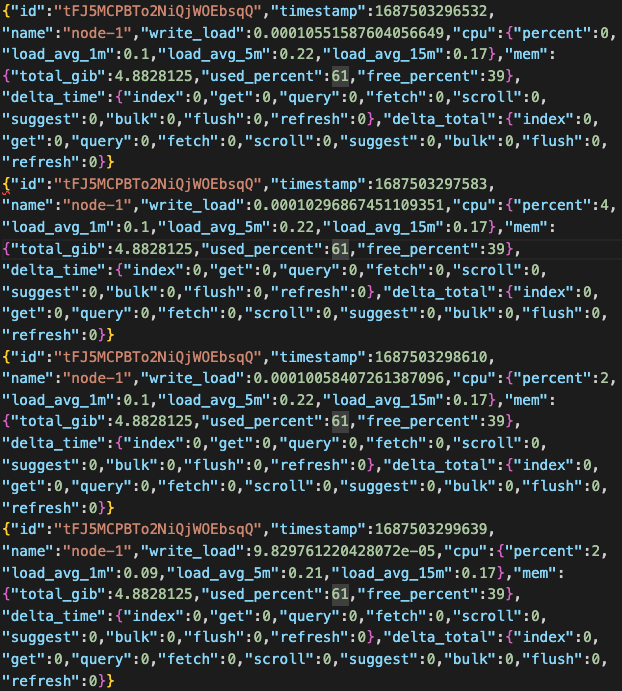
\includegraphics[width=0.8\textwidth]{chapter-4/mf-1.png}
  \caption{Hasil Pengujian Komponen \textit{Metrics Fetcher} Skenario 1}
  \label{fig:mf-1}
\end{figure}

\begin{figure}[h]
  \centering
  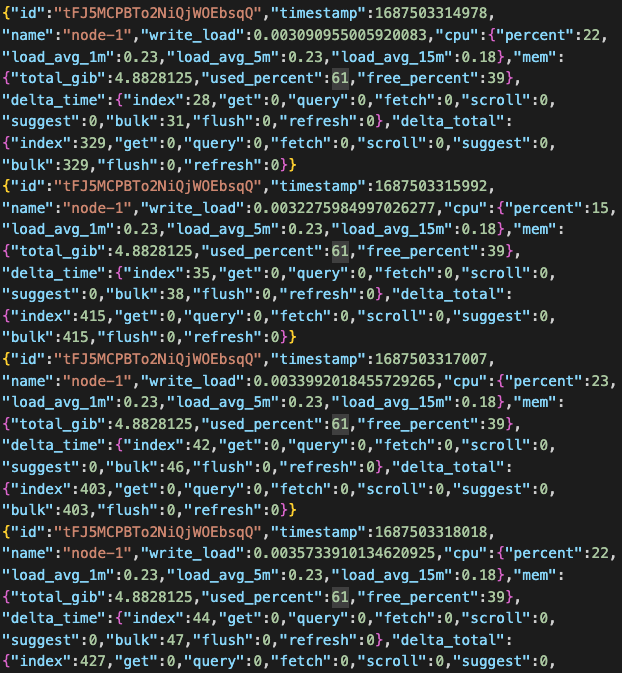
\includegraphics[width=0.8\textwidth]{chapter-4/mf-2.png}
  \caption{Hasil Pengujian Komponen \textit{Metrics Fetcher} Skenario 2}
  \label{fig:mf-2}
\end{figure}

\begin{figure}[h]
  \centering
  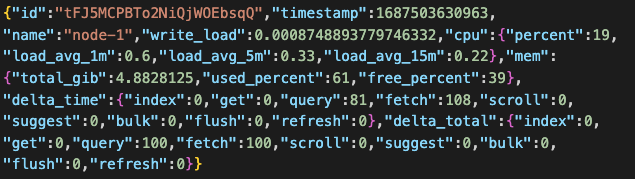
\includegraphics[width=0.8\textwidth]{chapter-4/mf-3.png}
  \caption{Hasil Pengujian Komponen \textit{Metrics Fetcher} Skenario 3}
  \label{fig:mf-3}
\end{figure}

Pengujian komponen \textbf{\textit{Metrics Fetcher}} sudah sesuai ekspektasi dan dapat dilanjutkan ke pengujian komponen lainnya.
% \subsubsection{Komponen \textbf{\textit{Predictor}}}
Komponen \textbf{\textit{Predictor}} dirancangkan terdiri dari 3 buah kelas, yaitu sebagai berikut.
\begin{enumerate}
    \item \textbf{\textit{Predict Component}}
    
    Kelas ini berfungsi untuk menyimpan sebuah model ARIMA untuk sebuah variabel. Kelas ini memanfaatkan kakas pandas, statsmodels dan pmdarima untuk melakukan tanggung jawabnya.

    \item \textbf{\textit{Predict Component Factory}}
    
    Kelas ini berfungsi untuk membuat objek \textbf{\textit{Predict Component}} sebanyak variabel yang ada. 

    \item \textbf{\textit{Predict Component Storage}}
    
    Kelas ini berfungsi sebagai aggregator objek \textbf{\textit{Predict Component}} yang telah dibuat oleh \textbf{\textit{Predict Component Factory}}. Kelas ini juga berfungsi untuk meneruskan sebuah aksi kepada semua objek \textbf{\textit{Predict Component}} yang ada. Contohnya, dengan memanggil \textit{forecast} atau \textit{update data}, maka operasi akan diteruskan ke semua objek \textbf{\textit{Predict Component}}.

\end{enumerate}

\begin{figure}[h]
    \centering
    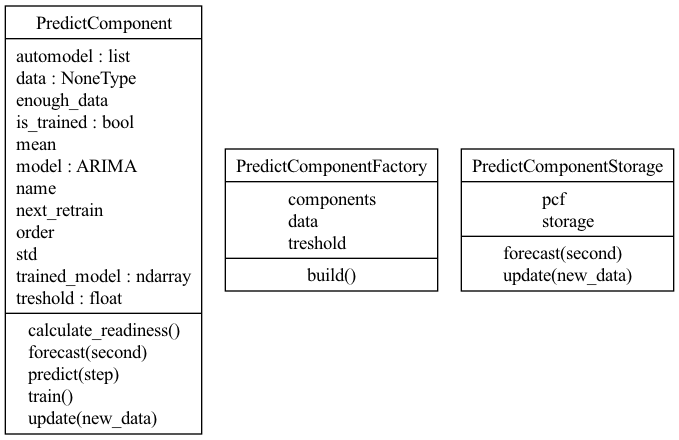
\includegraphics[width=0.8\textwidth]{chapter-4/predictor.png}
    \caption{Spesifikasi Kelas Penyusun Komponen \textit{Predictor}}
    \label{fig:predictor-spek}
\end{figure}

Secara umum, spesifikasi kelas bisa dilihat pada gambar \ref{fig:predictor-spek}. Kelas \textbf{\textit{Predict Component Storage}} akan membutuhkan \textbf{\textit{Predict Component Factory}} untuk membangun semua \textbf{\textit{Predict Component}} untuk setiap variabel yang ada. Setelah itu, terdapat operasi seperti meneruskan penambahan data serta meminta data prediksi ke setiap \textbf{\textit{Predict Component}}. Kelas ini akan digunakan oleh komponen \textbf{\textit{Flexible Control}} untuk lebih lanjutnya.
% \subsubsection{Komponen \textbf{\textit{Rule Manager}}}
Komponen \textbf{\textit{Rule Manager}} dirancangkan melakukan parsing terhadap file \textit{rule} yang telah diisi oleh pengguna serta menjadi aggregator untuk melakukan pengecekan \textit{rule} yang berlangsung serta memberi informasi data prediksi kapan saja yang dibutuhkan untuk melakukan pengecekan. Parsing komponen ini menggunakan format csv dan kondisi diekspresikan dengan sintaks python. Komponen akan mengonstruksi objek \textbf{\textit{Rule}} yang akan digunakan oleh komponen \textbf{\textit{Flexible Control}}. Spesifikasi dari kedua kelas tersebut dapat dilihat pada gambar \ref{fig:rule-spek}.

\begin{figure}[h]
    \centering
    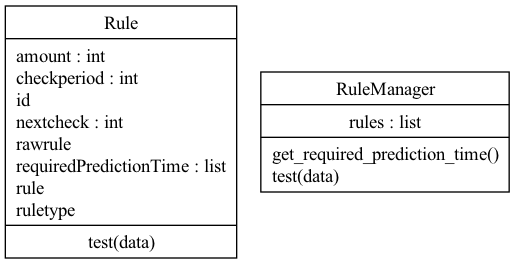
\includegraphics[width=0.8\textwidth]{chapter-4/rule.png}
    \caption{Spesifikasi Kelas Penyusun Komponen \textit{Rule Manager}}
    \label{fig:rule-spek}
\end{figure}

Sebuah \textit{rule} memiliki fungsi sebagai berikut.
\begin{enumerate}
    \item Memiliki sebuah kondisi yang akan dievaluasi dengan data prediksi pada waktu prediksi yang diinginkan. Contoh: kondisi \textit{throughput} untuk operasi X untuk 1 menit kedepan dan 5 menit kedepan lebih dari 1s, maka tingkatkan prosesor sebanyak 500m.
    \item Memiliki jumlah serta target kategori untuk diubah, dalam kasus ini pilihannya memori atau prosesor.
    \item Satuan untuk perubahan memori adalah dalam \textit{Mebibyte} atau MiB. Sedangkan untuk prosesor dalam satuan mili atau m.
    \item Sebuah \textit{rule} memiliki periode pengecekan sehingga tidak akan dicek secara terus menerus yang menyebabkan perubahan alokasi sumber daya terlalu cepat. Periode pengecekan dibuat dalam satuan sekon.
\end{enumerate}
% \subsection{Komponen \textit{Resource Controller}}

Seperti yang sudah dirancangkan sebelumnya, kelas ini menggunakan \textit{Kubernetes Client API} untuk mengubah alokasi sumber daya. Diimplementasikan dengan sistem antrian, sehingga jika sejumlah rule aktif secara bersamaan, maka akan dijalankan secara berurutan. Terdapat sebuah fungsi \textit{tick} yang akan berfungsi untuk mengeksekusi antrian. Contoh simpanan file antrian dapat dilihat pada gambar \ref{fig:ex-queue-rc}. File tersebut menyimpan status alokasi sumber daya pada saat itu, kapan melakukan perubahan pada antrian berikutnya dalam waktu UNIX dan antrian yang akan dieksekusi satu per satu.

\begin{figure}[h]
    \centering
    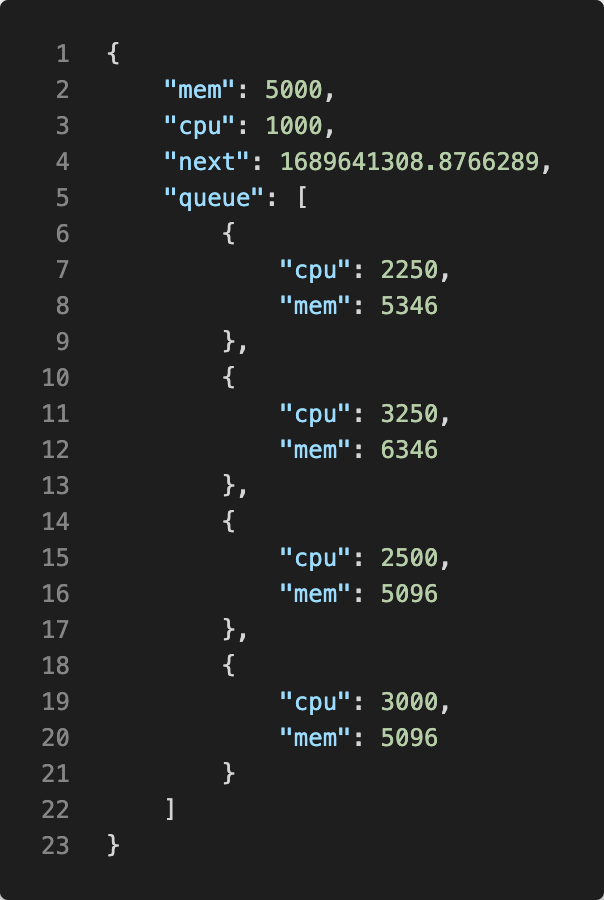
\includegraphics[width=0.45\textwidth]{chapter-4/rc-queue-ex.png}
    \caption{Contoh File Antrian Pengubahan Alokasi}
    \label{fig:ex-queue-rc}
\end{figure}

% TODO CONTOH SISTEM ANTRIAN
% % \subsection{Pengujian Sistem \textit{Flexible Control}}

Pada bagian ini akan dijelaskan tentang tujuan, skenario, hasil, dan analisis dari pengujian sistem sekaligus komponen \textbf{\textit{Flexible Control}}.

\subsubsection{Tujuan Pengujian}

Tujuan pengujian ini memastikan sistem \textbf{\textit{Flexible Control}} dapat berjalan dengan baik dan menghasilkan perilaku yang sesuai.

\subsubsection{Skenario Pengujian}

Pengujian terhadap komponen \textbf{\textit{Flexible Control}} dilakukan dengan beberapa skenario sebagai berikut serta ekspektasi dari pengujian yang dilakukan.
\begin{enumerate}
  \item \bfseries Sebuah \textit{rule} memenuhi kondisi untuk mengubah alokasi prosesor.\normalfont

        Prosesor akan berubah jumlahnya sesuai dengan \textit{rule} yang memenuhi kondisi. Perubahan pada spesifikasi \textit{pods} juga diekspektasikan mengikuti.

  \item \bfseries Sebuah \textit{rule} memenuhi kondisi untuk mengubah alokasi memori.\normalfont

        Prosesor akan berubah jumlahnya sesuai dengan \textit{rule} yang memenuhi kondisi. Perubahan pada spesifikasi \textit{pods} juga diekspektasikan mengikuti. Memory Used Percent akan menurun karena penambahan yang terjadi.
\end{enumerate}

\subsubsection{Hasil Pengujian dan Analisis}

Pengujian akan dilakukan dengan \textit{file rule} yang dapat dilihat pada gambar \ref{fig:ac-rule}. Terdapat dua buah \textit{rule} yang akan diuraikan sebagai berikut.

\begin{enumerate}
  \item Jika \textit{load average 1m} pada 10 detik kedepan diprediksikan diatas 0 maka akan ditambah alokasi prosesor sebesar 1000m atau sejumlah 1. Kondisi dari \textit{rule} sengaja dibuat seperti itu agar rule pasti terpenuhi.
  \item Jika \textit{memory used percent} pada 5 dan 10 detik kedepan diprediksikan diatas 60 maka akan ditambah alokasi memori sebesar 2048 mebibyte atau sejumlah 2 gibibyte (Gi). Kondisi dari \textit{rule} sengaja dibuat seperti itu agar rule pasti terpenuhi.
\end{enumerate}

Hasil dari pengujian skenario kedua dapat dilihat pada gambar \ref{fig:ac-mem}. Dan perubahan terhadap spesifikasi pods dapat dilihat pada gambar \ref{fig:ac-mem-kube}. Perubahan juga terjadi pada \textit{memory used percent} pada \textit{stream file} atau data yang ditarik oleh komponen \textbf{\textit{Metrics Fetcher}} dapat dilihat pada gambar \ref{fig:ac-mf-turun}.
Diikuti dengan hasil dari pengujian skenario pertama dapat dilihat pada gambar \ref{fig:ac-cpu}. Dapat dilihat bahwa prosesor berubah sesuai dengan ekspektasi. Perubahan pada spesifikasi \textit{pods} juga mengikuti perubahan prosesor yang dapat dilihat pada gambar \ref{fig:ac-cpu-kube}.

\begin{figure}[h]
  \centering
  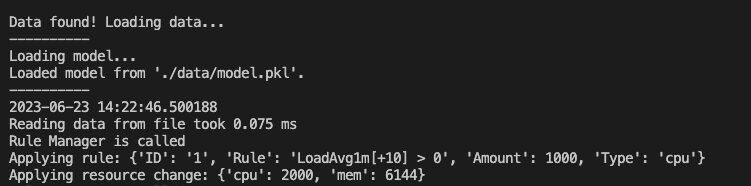
\includegraphics[width=0.8\textwidth]{chapter-4/ac-cpu.png}
  \caption{Hasil Pengujian Komponen \textit{Flexible Control} Skenario 1: Perubahan Prosesor}
  \label{fig:ac-cpu}
\end{figure}

\begin{figure}[h]
  \centering
  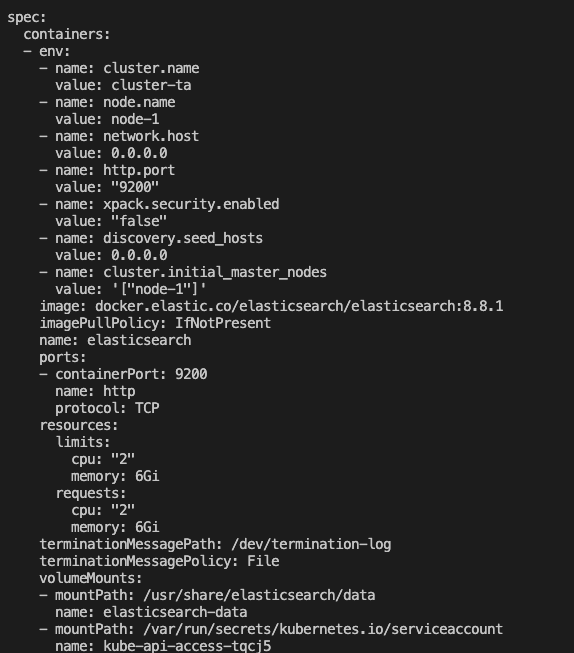
\includegraphics[width=0.8\textwidth]{chapter-4/ac-cpu-kube.png}
  \caption{Hasil Pengujian Komponen \textit{Flexible Control} Skenario 1: Perubahan Spesifikasi Kubernetes}
  \label{fig:ac-cpu-kube}
\end{figure}

\begin{figure}[h]
  \centering
  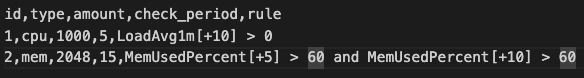
\includegraphics[width=0.8\textwidth]{chapter-4/ac-rule.png}
  \caption{File Rule untuk Pengujian Komponen \textit{Flexible Control}}
  \label{fig:ac-rule}
\end{figure}

\begin{figure}[h]
  \centering
  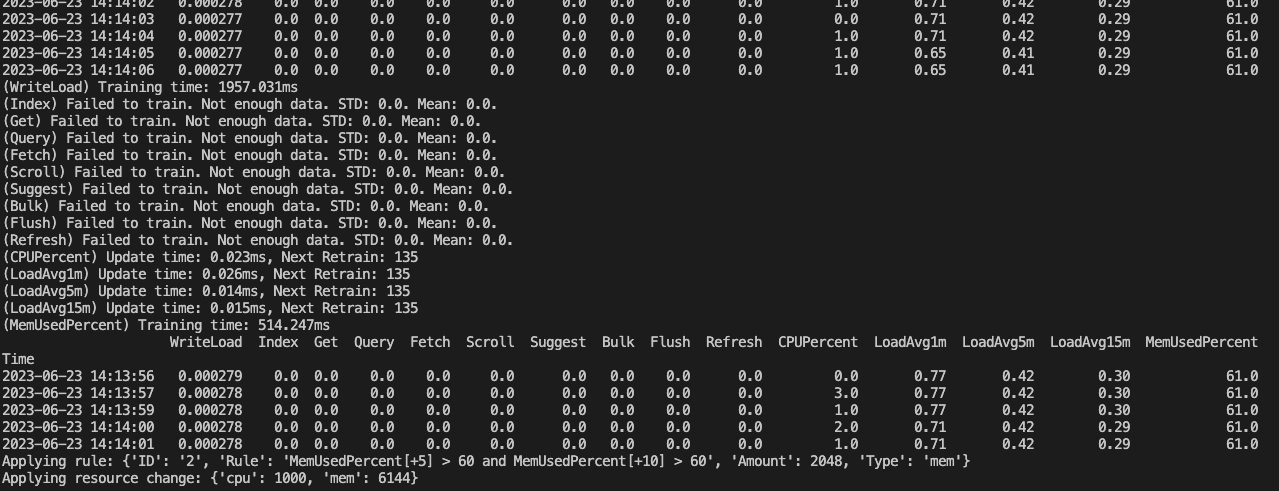
\includegraphics[width=1\textwidth]{chapter-4/ac-mem.png}
  \caption{Hasil Pengujian Komponen \textit{Flexible Control} Skenario 2: Perubahan Memori}
  \label{fig:ac-mem}
\end{figure}

\begin{figure}[h]
  \centering
  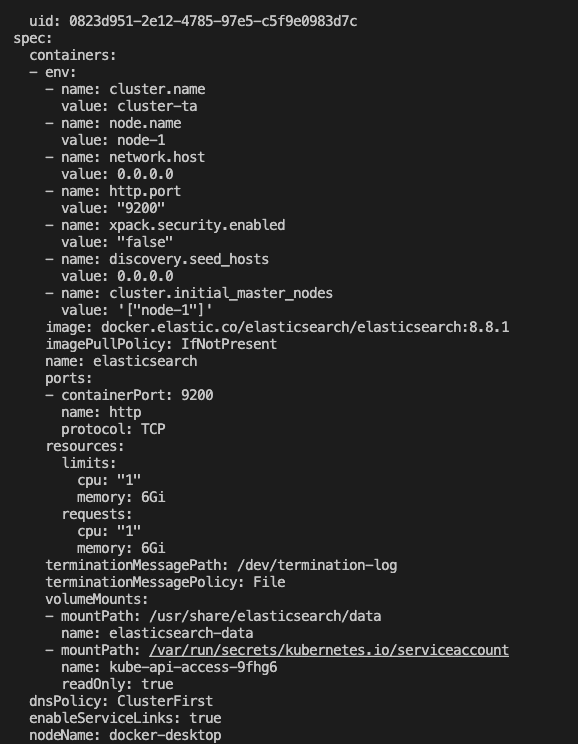
\includegraphics[width=0.8\textwidth]{chapter-4/ac-mem-kube.png}
  \caption{Hasil Pengujian Komponen \textit{Flexible Control} Skenario 2: Perubahan Spesifikasi Kubernetes}
  \label{fig:ac-mem-kube}
\end{figure}

\begin{figure}[h]
  \centering
  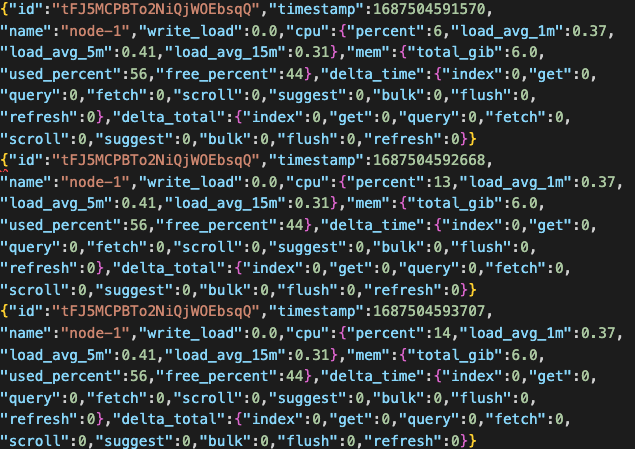
\includegraphics[width=0.8\textwidth]{chapter-4/ac-mf-turun.png}
  \caption{Hasil Pengujian Komponen \textit{Flexible Control} Skenario 2: Perubahan Memory Used Percent pada \textit{stream file}}
  \label{fig:ac-mf-turun}
\end{figure}

Pengujian komponen \textbf{\textit{Flexible Control}} sudah sesuai ekspektasi dan sistem dapat berjalan dengan baik.
% \subsection{Komponen Pendukung: Konfigurasi dan Utilitas}
\label{sec:komponen-pendukung}

Seperti yang sudah dijelaskan sebelumnya, terdapat konfigurasi yang dapat mengatur sistem. Konfigurasi yang dapat diatur dapat dilihat pada gambar \ref{fig:config-spek}.

\begin{figure}[ht]
  \centering
  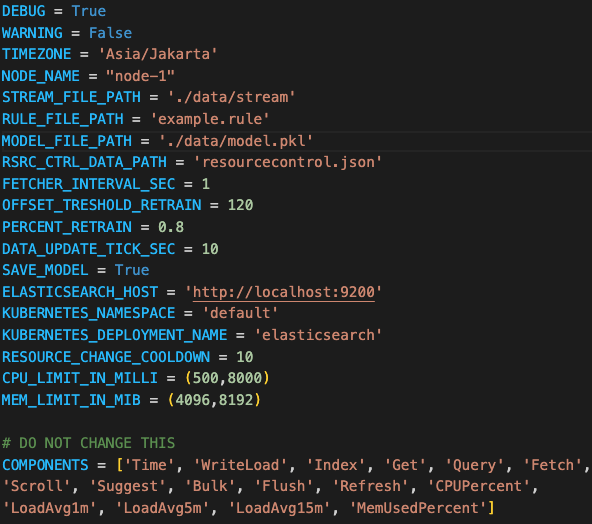
\includegraphics[width=0.8\textwidth]{chapter-4/config.png}
  \caption{Konfigurasi \textit{Flexible Control}}
  \label{fig:config-spek}
\end{figure}

Setiap konfigurasi tersebut mengatur perilaku dari sistem. Untuk setiap konfigurasinya, berikut adalah penjelasannya.

\begin{enumerate}
  \item \textbf{\textit{Debug}} dan \textbf{\textit{Warning}}

        Kedua \textit{flag} ini adalah untuk mematikan dan menyalakan pesan \textit{debug} dan \textit{warning}. Jika \textit{debug} dimatikan, maka program tidak akan mengirimkan pesan apapun selama berjalan.

  \item \textbf{\textit{Timezone}}

        Flag ini bertujuan untuk mengubah zona waktu yang digunakan oleh pandas karena data yang didapatkan dari \textit{Elastic Search} adalah berupa unix time sehingga akan dibaca secara \textit{default} menjadi UTC saat dikonversi.

  \item \textbf{\textit{Node Name}}, \textbf{\textit{Namespace}} dan \textbf{\textit{Deployment Name}}

        \textbf{\textit{Node Name}} adalah nama \textit{node} yang telah dikonfigurasi pada \textit{pods Elastic Search}. Nama harus sesuai karena \textbf{\textit{Metrics Fetcher}} akan mencari data untuk node dengan nama tersebut. Sedangkan, \textbf{\textit{Namespace}} dan \textbf{\textit{Deployment Name}} berkaitan dengan \textit{namespace} dan \textit{deployment Elasticsearch} dengan Kubernetes.

  \item \textbf{\textit{Elasticsearch Host}}

        \textit{Flag} ini berisikan target \textit{host} dari \textit{Elasticsearch}. Bertindak sebagai \textit{Base URL} untuk mengakses API \textit{Elastic Search}.

  \item \textbf{\textit{CPU Limit}} dan \textbf{\textit{Memory Limit}}

        Kedua limit ini digunakan untuk \textbf{\textit{Resource Controller}} mengubah alokasi sumber daya. \textit{Flag} ini berisikan \textit{tuple} dengan dua buah angka yang berguna sebagai batas bawah dan batas atas dari sumber daya bersangkutan. Satuan yang digunakan untuk prosesor adalah mili (m) sedangkan untuk memori adalah \textit{mebibyte} (MiB). Kedua batas ini bersifat inklusif.

  \item \textbf{\textit{File Path}}

        Seperti namanya, konfigurasi yang berkaitan dengan \textit{file path} berfungsi untuk mengatur tata letak file yang akan dibuat/dibaca oleh sistem.

  \item \textbf{\textit{Fetcher Interval}}, \textbf{\textit{Resource Change Cooldown}} dan \textbf{\textit{Data Update Tick Second}}

        \textbf{\textit{Fetcher Interval}} adalah interval komponen \textbf{\textit{Metrics Fetcher}} melakukan penarikan data. Lalu, \textbf{\textit{Resource Change Cooldown}} adalah waktu yang diperlukan oleh \textbf{\textit{Resource Controller}} untuk menunggu sebelum melakukan perubahan sumber daya. Terakhir, \textbf{\textit{Data Update Tick Second}} adalah interval yang digunakan oleh \textbf{\textit{Flexible Control}} untuk melakukan pembacaan data dari \textit{stream file}. \textbf{\textit{Data Update Tick Second}} harus lebih besar sama dengan \textbf{\textit{Fetcher Interval}} agar efisien. Satuan yang digunakan oleh ketiga \textit{flag} tersebut adalah detik.

  \item \textbf{\textit{Save Model}}

        \textit{Flag} ini berfungsi untuk mematikan penyimpanan model setiap kali model berubah. Jika \textit{flag} ini tidak dinyalakan, maka setiap kali sistem melakukan \textit{restart}, model prediksi akan diulang dari kosong.

  \item \textbf{\textit{Offset Treshold Retrain}} dan \textbf{\textit{Percent Retrain}}

        Dalam melakukan penambahan data, tidak setiap saat model akan di-\textit{retrain}. Saat tidak di-\textit{retrain}, model prediksi hanya melakukan update yang jauh lebih cepat namun tidak terlalu akurat. Terdapat sebuah angka yang akan menentukan kapan model harus di-\textit{retrain}. Hal ini diperlukan karena melakukan \textit{retrain} membutuhkan waktu yang lama terutama saat data sudah sangat besar. \textbf{\textit{Offset Treshold Retrain}} adalah angka yang menentukan kapan model harus di-\textit{retrain} berdasarkan jumlah data fixed. Sedangkan, \textbf{\textit{Percent Retrain}} adalah angka yang menentukan kapan model harus di-\textit{retrain} berdasarkan persentase jumlah data saat itu. Dengan persamaan \ref{eq:retrain-time}, \textbf{\textit{Offset Treshold Retrain}} adalah variable $c$ dan \textbf{\textit{Percent Retrain}} adalah variable $p$.
\end{enumerate}

Terdapat juga fungsi-fungsi utilitas yang akan membantu komponen-komponen yang telah dijelaskan sebelumnya, spesifikasi utilitas bisa dilihat pada gambar \ref{fig:util-spek}. Untuk setiap fungsinya, berikut adalah kegunaannya.

\begin{enumerate}
  \item \textbf{\textit{Save Model}}

        Fungsi ini akan menyimpan model yang telah dilatih ke dalam sebuah file. Digunakan kakas \textit{pickle} untuk melakukan hal ini.

  \item \textbf{\textit{Load Model}}

        Fungsi ini akan memuat model yang telah dilatih dari sebuah file. Digunakan kakas \textit{pickle} untuk melakukan hal ini.

  \item \textbf{\textit{Timings}}

        Fungsi adalah abstraksi untuk menghitung waktu eksekusi. Digunakan fungsi sebagai \textit{return value} agar lebih rapih ketika diperlukan banyak penghitungan waktu eksekusi.

  \item \textbf{\textit{Printd}}

        Fungsi ini hanyalah \textit{wrapper} dari fungsi \textit{print} pada Python untuk mengikuti aturan konfigurasi.

  \item \textbf{\textit{Read From File}}

        Fungsi ini digunakan untuk membaca \textit{stream file}. Fungsi ini digunakan oleh komponen \textbf{\textit{Flexible Control}} untuk membaca secara periodik, mentranformasikan dan mengirimkan data ke \textbf{\textit{Predict Component Storage}}.

  \item \textbf{\textit{To Vector}}

        Fungsi ini adalah fungsi transformasi format JSON (\textit{Java Syntax Object Notation}) yang ditulis ke \textit{stream file} menjadi sebuah \textit{numpy array} yang akan digunakan untuk membuat \textit{pandas dataframe}.

  \item \textbf{\textit{Create Dataframe}}

        Seperti namanya, fungsi ini membuat dataframe dari data yang telah dibaca dari \textit{stream file} dan sudah ditransformasikan dengan fungsi \textbf{\textit{to vector}}.

  \item \textbf{\textit{Extract Number From String}}

        Fungsi ini memanfaatkan regex untuk mengambil angka dari sebuah string.
\end{enumerate}

\begin{figure}[ht]
  \centering
  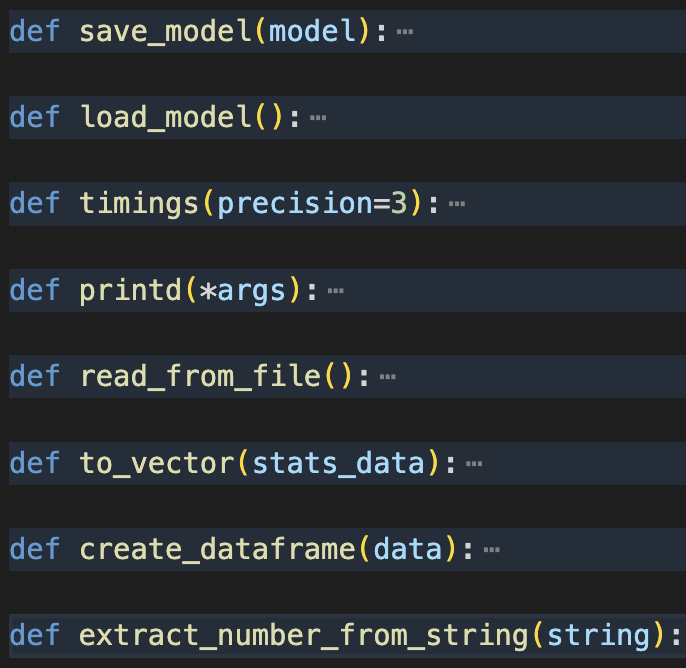
\includegraphics[width=0.6\textwidth]{chapter-4/utils.png}
  \caption{Spesifikasi Fungsi Utilitas Pendukung}
  \label{fig:util-spek}
\end{figure}

% \subsection{Penggunaan untuk \textit{Pods} dengan Aplikasi Lain}

% Sistem yang diimplementasikan juga dapat digunakan untuk pods lainnya. Tentunya dengan mengubah konfigurasi serta membuat \textbf{\textit{Metrics Fetcher}} khusus untuk aplikasi tersebut. Berikut adalah \textit{requirement} untuk dapat digunakan pada \textit{pods} lain.

% \begin{enumerate}
%   \item Aplikasi tersebut harus memiliki \textit{metrics} yang dapat diambil melalui suatu API, dapat berbentuk HTTP, GRPC atau yang lainnya. \label{item:requirement-general-1}
%   \item Aplikasi harus bisa mempunyai komponen untuk menghitung \textit{throuhgput} untuk setiap operasinya. \label{item:requirement-general-2}
% \end{enumerate}

% Ketika poin \ref{item:requirement-general-1} dan \ref{item:requirement-general-2} sudah terpenuhi, maka langkah-langkah yang harus dilakukan adalah sebagai berikut.

% \begin{enumerate}
%   \item Membuat komponen \textbf{\textit{Metrics Fetcher}} yang baru untuk aplikasi tersebut.

%         Dalam melakukan hal ini, transformasi sebaiknya diusahakan disesuaikan dengan struktur data yang sudah ada. Namun, jika ingin mengubah, maka harus melakukan pengubahan ekstra pada fungsi pemetaan \textit{metrics} yang ada pada komponen \textbf{\textit{Predictor}}.
%   \item Menyesuaikan konfigurasi dan fungsi pemetaan komponen \textbf{\textit{Predictor}}.

%         Tentunya, nama operasi akan berbeda serta detil-detil utilisasi umum akan berbeda sehingga diperlukan untuk mengubah dan menyesuaikan pada file konfigurasi.

%   \item Mengubah \textit{label selector kubernetes} pada komponen \textbf{\textit{Resource Controller}}

%         Karena sebelumnya dispesifikan ke aplikasi \textit{Elastic Search}, akibatnya, untuk mengubah ke aplikasi lain, perlu melakukan pengubahan \textit{label selector}.
% \end{enumerate}

% Setelah melakukan pengubahan tersebut, sistem sudah dapat digunakan untuk aplikasi lainnya.